%!TEX root=main.tex
\section{背景}
\label{clicknp:sec:background}

\subsection{软件网络功能的性能局限}

在诸如公共云的虚拟化环境的传统设备共享模型中,进出物理设备的所有网络I / O都专门在管理程序的主机软件分区中执行。 VM发送和接收的每个数据包都由主机网络堆栈中的虚拟交换机(vSwitch)处理。 接收数据包通常涉及管理程序将每个数据包复制到VM可见缓冲区,模拟到VM的软中断,然后允许VM的OS堆栈继续进行网络处理。 发送数据包类似,但顺序相反。 与非虚拟化环境相比,这种额外的主机处理:降低性能,需要对权限级别进行额外更改,降低吞吐量,增加延迟和延迟变化,并提高主机CPU利用率。

除销售虚拟机外,销售基础架构即服务(IaaS)的云供应商必须提供丰富的网络语义,例如具有客户提供的地址空间的私有虚拟网络,可扩展的L4负载平衡器,安全组和ACL ,虚拟路由表,带宽计量,QoS等。 这些语义非常复杂,而且变化太频繁,以至于在传统交换机硬件中大规模实现这些语义是不可行的。 相反,这些是在vSwitch中的每个主机上实现的。 这可以很好地适应服务器的数量,并允许物理网络简单,可扩展且速度非常快。

\textbf{列出性能数字。}

我们仍然根据我们仅使用主机内核运行我们的SDN堆栈的原始策略来评估所有选项,特别是像DPDK [18]这样的技术表明我们可以通过绕过OS网络堆栈来显着降低数据包处理成本 并在轮询模式下运行核心。 考虑到我们无法使ASIC满足我们的可编程性要求,这个选项击败了ASIC,但是如第3节所述,将内核烧录到VM托管成本的成本和性能开销足够高,即使是效率低下的多核SoC也是如此 更好的方法。

与其竞争对手一样,Azure作为IaaS产品直接向客户销售虚拟机,并竞争这些虚拟机的价格。我们在IaaS中的盈利能力是客户为虚拟机支付的价格与托管虚拟机的成本之间的差异。由于我们已经为每台服务器固定了成本,因此降低VM成本的最佳方法是将更多VM打包到每台主机服务器上。因此,大多数云通常在给定的2插槽(经济和性能标准)刀片上合理地部署最大数量的CPU核心。在撰写本文时,物理核心(2个超线程)的售价为0.10-0.11美元/小时1,或者最大潜在收入约为900美元/年,在服务器的生命周期内售价为4500美元(服务器通常持续3到5年)在我们的数据中心)。即使考虑到某些部分核心在任何时候都未售出,并且云通常为客户提供购买容量的折扣,与专用硬件相比,甚至使用一个物理核心进行主机网络也是相当昂贵的。我们的业务从根本上依赖于为每个主机销售尽可能多的内核到客户虚拟机,因此我们将竭尽全力减少主机开销。因此,应避免使用主机CPU内核运行高速SDN数据路径。

\subsection{硬件加速的选择}

传统上,微软与网络ASIC供应商(如英特尔,Mellanox,Broadcom等)合作,为Windows中的主机网络实现卸载 - 例如,在20世纪90年代的TCP校验和分段卸载[9],接收端扩展(RSS)[ 10]和虚拟机器队列(VMQ)[11]用于2000年代的多核可扩展性,以及最近无状态卸载用于Azure的虚拟网络方案的NVGRE和VxLAN封装在2010年[12]。事实上,GFT最初设计为由ASIC供应商实施,与SR-IOV一起作为精确匹配行动表,我们在业界广泛分享早期设计理念,看看供应商是否能满足我们的要求。随着时间的推移,我们对这种方法的热情逐渐降低,因为没有出现能够满足第3节中规定的所有设计目标和约束的设计。

SmartNIC供应商面临的一个主要问题是SR-IOV是一个全有或全无卸载的例子。如果在SmartNIC中无法成功处理任何所需的SDN功能,则SDN堆栈必须恢复为通过基于软件的SDN堆栈发送回流,几乎丧失了SR-IOV卸载的所有性能优势。

我们看到了几种不同的可能方向:网络交换机,GPU,ASIC,SoC,FPGA。


为了加速软件包处理,以前的工作已经提出使用GPU \cite {packetshader},专用网络处理器(NP)\cite {cavium,netronome} 和硬件交换机 \cite {duet}。
GPU主要用于图形处理,最近扩展到具有海量数据并行性的其他应用程序。 GPU更适合批量操作。 Han,\ etal~ \cite {packetshader},表明使用GPU可以实现40Gbps的分组交换速度。
但是,批量操作会导致高延迟。
例如,\cite {packetshader}中报告的转发延迟约为$200 \mu{}s$,比 \name{} 大两个数量级。
与GPU相比,FPGA更灵活,可以重新配置以捕获数据和流水线并行,这两者在NF中非常常见。
然而,NP专门用于处理网络流量并且具有许多硬连线网络加速器。
相比之下,FPGA是一种通用计算平台。
除了NF之外,FPGA在数据中心还有许多其他应用,使其更具吸引力
大规模部署 \cite {putnam2014reconfigurable}。
硬件交换机功能有限,其应用受到很大限制 \cite {duet}。


\subsubsection{用网络交换机实现网络功能}

\subsubsection{用 GPU 实现网络功能}

\subsubsection{基于 ASIC 的网卡}

用于SDN处理的定制ASIC设计提供了最高的性能潜力。然而,随着时间的推移,它们缺乏可编程性和适应性。特别是,需求规格与硅的到货之间的长时间跨度大约为1  -  2年,并且在这个范围内需求持续变化,使得新的硅已经落后于软件要求。 ASIC设计必须继续为服务器的5年生命周期提供所有功能(以我们的规模改造大多数服务器是不可行的)。全有或全无卸载意味着今天制定的ASIC设计规范必须满足未来7年的所有SDN要求。

ASIC供应商通常会添加嵌入式CPU内核来处理新功能。与其他NIC处理硬件相比,这些内核可能很快成为性能瓶颈。此外,随着新功能的增加,这些内核可能会随着时间的推移而增加处理负担,从而加剧了性能瓶颈。这些内核通常也通过NIC的固件更新进行编程,由ASIC供应商处理并减慢新功能的部署。

\subsubsection{基于多核 SoC 的网卡}

基于多核SoC的NIC使用大量嵌入式CPU内核来处理数据包,交换一些性能以提供比ASIC设计更好的可编程性。这些设计在10GbE NIC生成中得到广泛应用。有些像Cavium [13]那样使用通用CPU核心(MIPS,后来的ARM64),而其他像Netronome [14]和Tilera则使用特定的网络处理核心。在这个空间内,我们更多地推荐通用SoC  - 基于我们的评估,它们更容易编程(您可以采用标准的DPDK样式代码并在熟悉的Linux环境中运行)。令人惊讶的是,与类似的ASIC设计相比,这些在性能上没有太大的缺点。

但是,在40GbE及以上的更高网络速度下,核心数量显着增加。分散和收集数据包的片上网络和调度程序变得越来越复杂和低效。我们经常看到10μs或更多的延迟与将数据包送入核心,处理数据包以及退回到网络相关 - 延迟明显高于ASIC,并且具有更大的可变性。有状态流往往只映射到一个核心/线程,以防止在单个流中进行状态分片和无序处理。因此,单个网络流量性能没有太大改善,因为嵌入式CPU不会以与网络带宽相同的速度增加性能。这导致开发人员必须在多个流中分布流量的问题,如第3节中所讨论的,将更快网络的性能优势限制为仅最大并行工作负载。

SoC式网络卸载的未来也是值得怀疑的。在10GbE时,整个封装是可以容忍的,一些通用SoC内核就足够了。 40GbE需要近4倍的核心,尽管几个供应商仍然创造了可行的解决方案。尽管如此,具有基于软件的数据路径的40GbE部件已经出人意料地大,耗电量大且价格昂贵,并且它们对100GbE,200GbE和400GbE的可扩展性看起来很黯淡。

因此,虽然我们发现SoC方法具有熟悉的编程模型的优点,但在更高的网络速度下,单流性能,更高的延迟和更差的可扩展性使我们寻找另一种解决方案。



\textbf{需要合并:
软件NF具有极大的灵活性和可扩展性。
早期研究主要集中在基于软件的数据包转发 \cite {routebricks,Egi:2008:THP:1544012.1544032}。
他们表明,多核x86 CPU可以以每服务器10Gbps的速度转发数据包,并且可以通过集群更多服务器来扩展容量。
最近,许多系统被设计用于实现各种类型的NF \cite {comb,Greenhalgh:2009:FPR:1517480.1517484,martins2014clickos}。
同样,所有这些系统都利用CPU中的多核并行性来实现每台机器接近10Gbps的吞吐量,并在需要更高容量时向外扩展以使用更多机器。
Ananta \cite {ananta}是一个部署在Microsoft数据中心的软件负载均衡器,用于提供云规模的负载均衡服务。
虽然软件NF可以扩展以提供更多容量,但这样做会在CAPEX和OPEX中增加相当大的成本 \cite {ananta,duet}。}



\subsubsection{基于 FPGA 的网卡}
\label{clicknp:subsec:fpga}
% Focus on FPGA architecture

顾名思义,FPGA(Field Programmable Gate Array)是\textit {逻辑门}的海洋。
FPGA的基本构建块是\textit {逻辑元件(LE)},它包含一个查找表(LUT)和一些寄存器。
LUT可以编程为计算任何组合逻辑,寄存器用于存储状态。
除基本LE外,FPGA还包含用于存储数据的Block RAM(BRAM)和用于复杂算术运算的数字信号处理(DSP)组件。
通常,FPGA通过PCIe附加板连接到PC,PCIe附加板也可能包含数千兆字节的DRAM和其他通信接口,例如10G / 40G以太网端口。
图\ref{clicknp:fig:fpga}显示了FPGA板的逻辑图。

\begin{figure}[t]
\centering
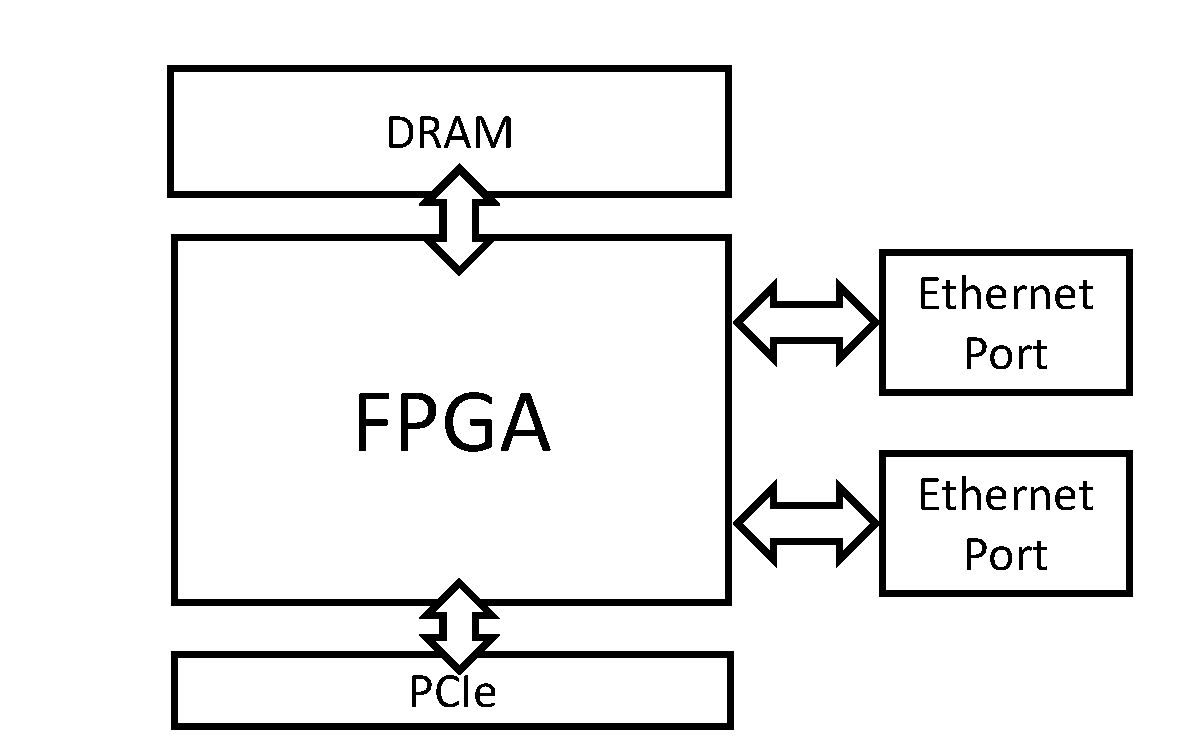
\includegraphics[width=0.6\textwidth]{fpga-board.pdf}

\caption{FPGA板的逻辑图。}
\label{clicknp:fig:fpga}

\end{figure}

%
% we need to make more points here: parallelism, memory hierarchy, or code?
%

与CPU或GPU相比,FPGA通常具有更低的时钟频率和更小的存储器带宽。
例如,FPGA的典型时钟频率约为200MHz,比CPU慢一个数量级(2至3~GHz)。
同样,FPGA的单块存储器或外部DRAM的带宽通常为2至10~GBps,而内存带宽约为Intel XEON CPU的40~GBps,GPU为100~GBps。
但是,CPU或GPU只有有限的内核,这限制了并行性。 FPGA内置了大量的并行性。
现代FPGA可能拥有数百万个LE,数百个K位寄存器,数十个M位BRAM和数千个DSP模块。从理论上讲,它们中的每一个都可以并行工作。
因此,FPGA芯片内部可能会同时运行数千个并行的``\textit {核}''。
虽然单个BRAM的带宽可能有限,但如果我们并行访问数千个BRAM,则总内存带宽可以是多TBps!
因此,为了实现高性能,程序员必须充分利用这种大规模的并行性。

传统上,FPGA使用诸如Verilog和VHDL之类的HDL进行编程。
这些语言水平太低,难以学习,编程也很复杂。
因此,大型软件程序员社区已经远离FPGA多年了~\cite {bacon2013fpga}。
为了简化这一点,许多高级综合(HLS)工具/系统已经在工业界和学术界开发,试图将高级语言(主要是C)的程序转换为HDL。
但是,正如我们将在下一小节中所示,它们都不适合网络功能处理,这是本工作的重点。

\subsection{基于 FPGA 的网络功能编程}

我们的目标是利用FPGA加速构建一个多功能,高性能的网络功能平台。这样的平台应满足以下要求。

\textbf {灵活性。} 平台应该\textit {完全使用高级语言编程。}
开发人员使用高级抽象和熟悉的工具编程,并具有类似的编程经验,就像在多核处理器上编程一样。
我们相信这是使大多数软件程序员可以使用FPGA的必要条件。

\textbf {模块化。} 我们应该支持\textit {模块化架构}进行数据包处理。以前关于虚拟化NF的经验表明,正确的模块化架构可以很好地捕获数据包处理中的许多常见功能~\cite {kohler2000click,martins2014clickos},使它们易于在各种NF中重用。

\textbf {高性能和低延迟。} 数据中心的NF应该以40 / 100~Gbps的线路速率处理大量数据包,具有超低延迟。以前的工作已经显示~\cite {rollback-mb},即使NF添加的几百微秒的延迟也会对服务体验产生负面影响。

\textbf {支持联合CPU / FPGA数据包处理。} 我们说FPGA不是灵丹妙药。
正如之前在\S \ref {clicknp:subsec:fpga} 中讨论的FPGA架构所推断的那样,并非所有任务都适用于FPGA。例如,自然顺序的算法和具有非常大的内存占用和低局部性的处理应该在CPU中处理得更好。
此外,FPGA具有严格的区域约束。
这意味着您无法将任意大的逻辑放入芯片中。
在没有数据平面中断的情况下动态交换FPGA配置非常困难,因为重新配置时间可能需要几秒到几分钟,具体取决于FPGA的大小。
因此,我们应该支持CPU和FPGA之间的细粒度处理分离。这需要CPU和FPGA之间的高性能通信。


现有的FPGA高级编程工具都不能满足上述所有要求。
大多数HLS工具,例如 Vivado HLS~\cite{vivado},只是HDL工具链的辅助工具。
这些工具不是直接将程序编译成FPGA映像,而是仅生成硬件模块,即IP核,必须手动嵌入在HDL项目和连接到其它HDL模块,这是大多数软件程序员无法完成的任务。

但是,Altera OpenCL可以直接将OpenCL程序编译为FPGA~ \cite {aoc}。
但是,OpenCL编程模型直接源自GPU编程,并且不是用于数据包处理的模块化。
此外,OpenCL不支持CPU和FPGA之间的联合数据包处理:
首先,主机程序和FPGA内核之间的通信必须始终通过板载DDR内存。 这增加了非平凡的延迟,并且还导致板载内存成为瓶颈。
其次,OpenCL内核函数需要宿主机上的软件程序显式\textit {调用}。
在内核终止之前,主机程序无法控制内核行为,例如设置新参数,也不能读取任何内核状态。
但是NF面临着连续的数据包流,应该始终在运行。

FPGA是一项成熟的技术,最近已经部署用于加速数据中心服务,包括网络功能 \cite {putnam2014reconfigurable,smartnic,rubow2010chimpp,lavasani2012compiling}。
众所周知,FPGA的可编程性很低,有丰富的前人工作提供了高级编程抽象 \cite {bluespec,auerbach2010lime,bacon2013fpga,singh2011implementing,bachrach2012chisel,wester2015transformation}。
Gorilla \cite {lavasani2012compiling} 为FPGA上的数据包交换提出了一种特定于域的高级语言。
然而,Chimpp \cite {rubow2010chimpp} 试图将Click模型引入HDL来开发模块化路由器。
\name 沿此方向工作,与以前的工作互补。
\name 致力于数据中心的NF,通过提供高度灵活的模块化架构和利用商业HLS工具解决可编程性问题。

Click2NetFPGA~\cite {Click2NetFPGA}通过直接将Click模块化路由器〜\ cite {kohler2000click}程序编译到FPGA中来提供模块化架构。
然而,\cite {Click2NetFPGA}的性能比我们在本文中报告的要低得多(两个数量级),因为它们的系统设计存在几个瓶颈(例如,内存和数据包I / O),它们也是 错过几个重要的优化以确保完全流水线处理(如\S \ref {clicknp:sec:optimization}中所述)。
此外,\cite {Click2NetFPGA}不支持FPGA / CPU联合处理,因此无法在数据平面运行时更新配置或读取状态。



在下面,我们将介绍\name{},一种新颖的FPGA加速网络功能平台,满足上述四个要求。

\egg{
Today's data centers rely on a wide range of network functions to implement network virtualization, ensure security (e.g. firewalls and intrusion detection/prevention systems), perform measurements and improve performance (e.g. traffic scheduling). As data centers are moving towards 40 Gbps bandwidth at end hosts, where the line-rate is 60 M packets per second for minimum-sized packets, higher throughput requirement is imposed upon network processors. Furthermore, as data center services are evolving rapidly, programmability becomes indispensable for network processors. However, existing network processors has a large mismatch to the performance and programmability requirements.

\subsection{Architectures for Network Processors}

Network processors based on general-purpose CPUs such as ClickOS \cite{martins2014clickos} enjoy good programmablity, modularity and composabilty, but the packet forwarding performance of a single core could not keep up with 10 Gbps line rate for minimum-sized packets, even before any network function is plugged in. Because CPU instructions are executed one-by-one and have low parallelism, packet processing performance would drop further as more network functions are added. If a CPU-based network processor is added bump-in-the-wire, there will be 10s of microseconds additional end-to-end latency \cite{martins2014clickos} which is one magnitude higher than the switching fabric. In network virtualization scenario, if packet encapsulation and decapsulation is done at end hosts, as in the case of virtual switch, NIC offloading mechanisms including Large Send Offload (LSO) and Large Receive Offload (LRO) have to be disabled, which has a huge impact on TCP performance \cite{yoshino2008performance}.

ASICs are known to be high-performance, but the network functions are fixed. Commodity switching ASICs typically have a pipeline of network functions \cite{broadcomethernet}, where each function can be configured via registers and a match table based on TCAM or memory. Some ASICs provide flexible OpenFlow-like match-action tables \cite{broadcomopenflow}, but the packet parser is fixed (we could not support new packet header and shim layer formats), actions are not extensible and the order of network functions in the pipeline is not reconfigurable.

GPUs are widely used as co-processors for computing-intensive tasks, but its SIMD (Single-Instruction Multiple-Data) programming model does not fit network processing, where different types of packets may take various execution flows. The high power consumption, high latency of batch processing and inability to receive and send network packets without CPU intervention are also factors that render GPU-based network processor infeasible in data centers.

Fortunately, reconfigurable hardware is an architecture that provides both programmability, high performance and power efficiency for certain workloads. FPGA (field programmable gate arrays) is the most prominent example of reconfigurable hardware. FPGAs can implement arbitrary logic function and utilize distributed on-chip registers and SRAM to exploit bit-level and task-level parallelism, therefore stream processing pipelines would not ``hit the memory wall'' as in Von Neumann architecture \cite{bacon2013fpga}. FPGA has shown potential in accelerating many workloads in cloud \cite{putnam2014reconfigurable}. Moreover, Moore's law is still working in FPGA industry, because the fabrication technology of FPGA is currently several generations behind the CPU industry [citation required].

\subsection{FPGA Programming Challenge}

Despite FPGA's potential in network processing, the programmablity of FPGA is traditionally provided by hardware description languages (HDL) such as Verilog, which requires hardware knowledge and are much harder to program and debug than higher-level languages such as C/C++. Thus, existing FPGA-based network processors such as NetFPGA \cite{lockwood2007netfpga} are hard to program for software engineers.

Many works, e.g. OpenFlow \cite{mckeown2008openflow}, P4 \cite{bosshart2014p4} and SDNet \cite{xilinxsdnet}, provides the programmability by abstracting a set of primitives in network processing and defining a high-level programming language to compose the primitives. This direction has proved effective, but the programmability is limited to a set of pre-defined actions, which could not keep pace with rapid development of data center network functions. Our work strive to make the primitives extensible for software engineers.

Fortunately, several frameworks have been proposed to provide abstractions for generic FPGA programming. Examples of such works include Xilinx Vivado HLS (High Level Synthesis) \cite{feist2012vivado} based on C/C++, Altera SDK for OpenCL \cite{czajkowski2012opencl} based on C-like OpenCL and IBM Lime \cite{auerbach2010lime} based on Java.

However, FPGA has a completely different architecture than general-purpose CPUs. For software programmers that bear Von Neumann model in mind, the compilers may generate surprisingly poor hardware logic for reasonable code in high-level language. For example, Click2NetFPGA \cite{Click2NetFPGA} uses LLVM and HLS tools to compile optimized Click C++ code into HDL, but the resulting FPGA-based router can only process 178 K pps (packets per second) for 98B packets, and 215 Mbps for large packets, which is 30 -- 50x slower than a CPU core in ClickOS \cite{martins2014clickos}. The bottleneck for small packets is the IP header checking stage \cite{Click2NetFPGA} because this stage is not fully pipelined; the bottleneck for large packets is the byte-wide shared memory \cite{Click2NetFPGA}, indicating a shared-memory design suitable for Von Neumann model would yield poor performance on FPGA.

FPGA has millions of logic gates with 10x slower clock rate than CPU, thousands of distributed fast SRAMs each with only KB capacity, and a large DRAM with 10x lower throughput than DRAMs in CPU architecture. Consequently, exploiting both spatial and temporal parallelism is crucial to unleashing the performance of FPGA. In network stream processing, most operations are independent of each other and therefore can be either parallelized (spatial) or pipelined (temporal), so that each stage of the pipeline can process different packets in parallel.

\subsection{Design Goals}
\label{clicknp:subsec:designgoals}

We highlight several design goals for our ClickNP framework to enable software engineers to write efficient network applications.

\smalltitle{Modularity.} Modularity is one key feature that improves parallelism, since modules do not have shared state and can run in parallel by nature. Borrowing the concepts from Click modular router \cite{kohler2000click}, \textit{elements} are basic building blocks of network functions. Elements run asynchronously and are connected via uni-directional \textit{channels}. The network processing pipeline is a data flow graph of elements and channels, starting from Ethernet receivers and ending at Ethernet transmitters.

\smalltitle{Line-rate throughput.} To allow efficient processing of packet content, an Ethernet packet is split into 32-byte \textit{flits} before feeding into elements. In the worst case, when 69-byte packets are received back-to-back, the line rate would be 40G / 8 / (69+20) = 56.18 Mpps, which splits into 56.18M * 3 = 168.54M flits. Every clock cycle an element reads at most one flit and outputs zero or one flit. This means any FPGA pipeline with clock frequency lower than 168.54 MHz would not be able to achieve line rate. If we waste a cycle between every two packets, the minimum clock frequency would be 224.72 MHz. However, on Stratix V FPGA platform \cite{stratix2012device}, non-trivial hardware logic that accesses registers and local memory can hardly run higher than 200 MHz. Therefore no idle cycles are allowed in elements processing packet content. First, the framework should provide abstractions for programmers to develop fully pipelined network functions. Second, as full compilation of a FPGA program may take hours, the framework should give performance warnings in an early compilation stage if the code cannot be fully pipelined.

\smalltitle{Code reuse.} Many network applications share a common set of elements, for example packet parser, lookup tables and packet modifications. Code of these elements should be reusable and elements should be composable. Software engineers should be able to write many network applications simply by connecting elements in the library.

\smalltitle{Debugging support.} First, as HDL (e.g. Verilog) simulation and debugging is both time consuming and requires extensive hardware knowledge, the framework should be able to compile OpenCL-based ClickNP programs to native x86 code for emulation, and provide traffic generators and receivers to test functionality. Second, as CPU is neither capable of sending or receiving packets at 60 Mpps, we need a FPGA-based network benchmark suite to perform stress testing on the network processor.

\smalltitle{Separation of control plane and data plane.} On one hand, our throughput requirement requires most network packets to be processed through the reconfigurable hardware without any CPU intervention. On the other hand, SDN and NFV applications are usually complicated and have external dependencies. Therefore a clear interface between the control plane and the data plane is mandatory, where data plane programs are written within ClickNP framework and target massive parallelism, and control plane programs need only slight modifications to call our host library and perform on-the-fly reconfigurations.

\smalltitle{Host communication.} Network processors require low-latency and high-throughput interactions with the host machine. In SDN and NFV applications, FPGA needs to send unknown packets to the controller and request a new forwarding rule to be inserted into FPGA. The round-trip time should be as low as possible to reduce end-to-end flow establish time. In packet replay and capture applications, FPGA needs to receive or send Gigabytes of packets from or to the host machine without using the network adapter.

We design ClickNP to meet the above design goals with Catapult FPGA \cite{putnam2014reconfigurable} and Altera OpenCL \cite{singh2011implementing}. In the next section, we will describe the FPGA and OpenCL components, and how we build a toolchain that abstracts away hardware specific details.
}

\egg{
\subsection{FPGA in datacenter}

Conventionally, datacenter operators largely relied on the performance improvements in general-purpose servers
to improve the operation efficiency. This performance improvement rate of servers 
has considerably slowed down recently due to the power limitations~\cite{putnam2014reconfigurable, more-citation}.
This has motivated the adoption of \textit{accelerator} that can be specialized to certain workloads to get efficiency gains.
However, the non-programmable ASIC-based accelerators are undesirable for datacenters due to following two reasons:
Firstly, datacenter operators prefers homogeneous server configurations to minimize the management overhead and also provide
a consistent platform that applications can rely on.
Secondly, services in datacenters evolve extremely rapidly. Waiting for the long release cycle of ASIC chips is undesirable.
%
Therefore, it requires a flexible accelerator that can potentially speed up many applications.
%
GPU and FPGA are two predominate technologies that satisfy this requirement.

% comparison between GPU and FPGA
% power efficiency
Compared with GPU, FPGA is more power efficient. For example, the latest NIVDIA xxx consumes xxx W power, while a high-end
Altera Stratix V consumes xxx W power ( J per op?) \knote{need a citation}. 
% versatile 
Further, FPGA is more versatile. While GPU is mainly designed to achieve \textit{data parallelism} with SPMD (single program, multiple data), 
FPGA can easily achieve both data parallelism and \textit{task parallelism} as different block of LEs can be independently configured to
implement different processing.  
% I/O
Finally, FPGA supports various I/O interface. Normally, GPU can only communicate with PC memory through PCIE bus. 
But FPGA can input or output data from many interfaces like network ports, and is more suitable for processing these 
I/O streams. 

FPGA is a mature technology and becomes inexpensive. A large scale deployment of FPGA in Microsoft datacenter shows 
that a high-end FPGA board increases the total cost of ownership (TCO) of a server by less than 30\%, but can double 
the Bing search efficiency~\cite{putnam2014reconfigurable}.
%
In this paper, we focus on using FPGA to accelerate network functions that are essential to our datacenter networks.
}

\egg{
\smalltitle{inexpensive}

Why I need this as background:
\begin{itemize}
\item Price issue?
\item Power?
\item Transition to FPGA for network functions?
\end{itemize}
}
